\documentclass[preprint,12pt,a4paper]{elsarticle}

\usepackage{amssymb}
\usepackage{amsmath}
\usepackage{hyperref}
\usepackage{tikz}
\usetikzlibrary{arrows.meta, positioning, calc}
\usepackage{booktabs}
\usepackage[table]{xcolor}
\setlength{\parindent}{0pt}

\definecolor{tableShade}{gray}{0.93}

\journal{SoftwareX}

\begin{document}
\renewcommand{\labelenumii}{\arabic{enumi}.\arabic{enumii}}

\begin{frontmatter}

\title{DecisionDB: Diagnostic Infrastructure for Representational Dependence in Discrete Outcome Pipelines}

\author[label1]{Gil Raitses}
\address[label1]{gilraitses@gmail.com}

\begin{abstract}
DecisionDB is a Python library for logging, replaying, and auditing how discrete outcomes depend on representational choices in analytical pipelines. It formalizes decision-valued maps: mappings from representation families to discrete decision identities under fixed data snapshots and fixed computational engines. All entities are content-addressed via SHA-256, stored in SQLite, and linked through a five-table relational schema. A five-stage sweep protocol supports systematic representational variation, and a replay verification procedure confirms deterministic recovery of persisted identifiers. DecisionDB makes representational dependence empirically testable without introducing performance targets or learning dynamics.
\end{abstract}

\begin{keyword}
representational dependence \sep decision identity \sep reproducibility \sep content addressing \sep diagnostic infrastructure \sep analytical pipelines
\end{keyword}

\end{frontmatter}

\section*{Metadata}
\label{}

\begin{table}[!h]
\begin{tabular}{|l|p{6.5cm}|p{6.5cm}|}
\hline
\textbf{Nr.} & \textbf{Code metadata description} & \textbf{Metadata} \\
\hline
C1 & Current code version & v0.1.0 \\
\hline
C2 & Permanent link to code/repository used for this code version & \url{https://github.com/GilRaitses/decisiondb} \\
\hline
C3 & Permanent link to Reproducible Capsule & -- \\
\hline
C4 & Legal Code License & MIT License \\
\hline
C5 & Code versioning system used & git \\
\hline
C6 & Software code languages, tools, and services used & Python 3, SQLite \\
\hline
C7 & Compilation requirements, operating environments \& dependencies & Python 3.9+, no external dependencies beyond the standard library \\
\hline
C8 & If available Link to developer documentation/manual & \url{https://github.com/GilRaitses/decisiondb/tree/main/decisiondb} \\
\hline
C9 & Support email for questions & gilraitses@gmail.com \\
\hline
\end{tabular}
\caption{Code metadata (mandatory)}
\label{codeMetadata}
\end{table}


\section{Motivation and significance}

Analytical pipelines in scientific, engineering, and policy settings produce discrete outcomes: a selected route, a diagnostic label, a risk classification. These outcomes depend on representational choices (how data is encoded, what features are weighted, which aggregation rules are applied) in ways that are rarely recorded or tested. Small changes to such choices can induce qualitatively different outcomes, even when the underlying data and computation are unchanged.

Current practice treats representational choices as incidental implementation details. When instabilities surface, they are typically discovered after deployment or during post-hoc audits, because no infrastructure existed to make them visible earlier. Existing approaches address related problems from different angles: specification curve analysis~\cite{simonsohn2020specification} and multiverse analysis~\cite{steegen2016increasing} characterize how continuous effect estimates vary across analytic specifications; global sensitivity analysis~\cite{saltelli2008global} decomposes output variance with respect to input variation; underspecification analysis~\cite{damour2022underspecification} documents divergent predictor behavior under distribution shift; and provenance systems such as W3C PROV~\cite{moreau2013prov} and MLflow~\cite{zaharia2018accelerating} track derivation history and experimental artifacts.

DecisionDB addresses a gap among these: it isolates representational variation as a first-class experimental variable and tracks its effect on \emph{discrete} outcome identity under fixed snapshots and engines. The object of analysis is a partition of representation space into persistence regions and boundaries, not a distribution of continuous metrics. The software enables users to systematically sweep representation parameters, log all artifacts with content-addressed identifiers, and verify replay determinism without re-executing engines.


\section{Software description}

\subsection{Software architecture}

DecisionDB is organized as a Python package with seven modules: \texttt{core} (canonical serialization, content-addressed ID generation, entity schemas), \texttt{decision} (equivalence policy management, decision extraction), \texttt{engine} (abstract engine adapter protocol), \texttt{store} (SQLite persistence with append-only writes), \texttt{sweeps} (sweep plan definition and five-stage execution), \texttt{replay} (verification of persisted identifiers), and \texttt{viz} (categorical visualization with enforced constraints against performance metrics).

The central abstraction is a decision-valued map $f\colon \mathcal{R} \to \mathcal{D}$, where $\mathcal{R}$ is a family of representations over a fixed snapshot and $\mathcal{D}$ is a set of discrete decision identities. Figure~\ref{fig:pipeline} illustrates the pipeline.

\begin{figure}[t]
  \centering
  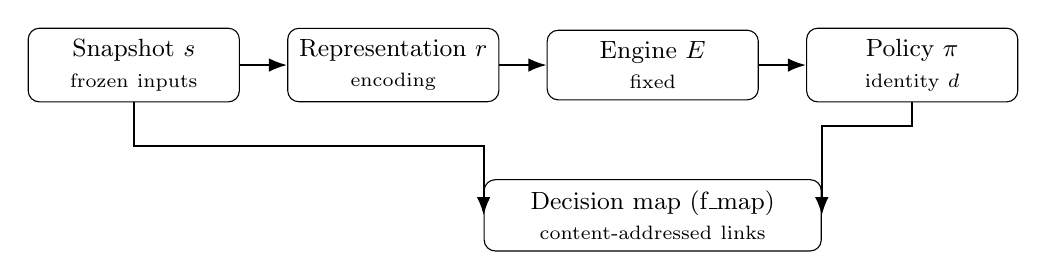
\begin{tikzpicture}[
    node distance=6mm,
    box/.style={draw, rounded corners, align=center, inner sep=4pt, text width=24mm, font=\small},
    arrow/.style={-Latex, thick}
  ]
  \node[box] (snap) {Snapshot $s$\\{\scriptsize frozen inputs}};
  \node[box, right=of snap] (rep) {Representation $r$\\{\scriptsize encoding}};
  \node[box, right=of rep] (eng) {Engine $E$\\{\scriptsize fixed}};
  \node[box, right=of eng] (pol) {Policy $\pi$\\{\scriptsize identity $d$}};
  \node[box, below=10mm of eng, text width=40mm] (map) {Decision map (f\_map)\\{\scriptsize content-addressed links}};
  \draw[arrow] (snap) -- (rep);
  \draw[arrow] (rep) -- (eng);
  \draw[arrow] (eng) -- (pol);
  \draw[arrow] (pol.south) -- ++(0,-0.3) -| (map.east);
  \draw[arrow] (snap.south) -- ++(0,-0.55) -| (map.west);
  \end{tikzpicture}
  \caption{Decision-valued mapping pipeline. A frozen snapshot is encoded into a representation, consumed by a fixed engine, and reduced to a discrete decision identity via an equivalence policy. The decision map materializes these links using content-addressed identifiers.}
  \label{fig:pipeline}
\end{figure}

\textbf{Content addressing.} All identifiers are computed deterministically: the entity payload is serialized to canonical JSON (sorted keys, no whitespace, floats as strings), hashed with SHA-256, truncated to 16 hex characters, and prefixed by type (\texttt{snap\_}, \texttt{repr\_}, \texttt{run\_}, \texttt{dec\_}, \texttt{pol\_}).

\textbf{Schema.} Five SQLite tables store the core entities: \texttt{snapshots} (frozen input state), \texttt{representations} (deterministic encodings with factory version), \texttt{engine\_runs} (execution records with pinned engine version and config hash), \texttt{decisions} (discrete identities with equivalence policy version), and \texttt{f\_map} (the materialized decision-valued map, keyed by representation and engine run). All writes are append-only and idempotent via \texttt{INSERT OR IGNORE}.

\textbf{Equivalence policies.} Each policy specifies a hash source (which output field carries decision-relevant content), a canonicalization rule, and a match rule. The policy is itself content-addressed, so changing the policy produces new decision identifiers downstream.

\subsection{Software functionalities}

\textbf{Five-stage sweep protocol.} (1)~Freeze a snapshot and assign a content-addressed identifier. (2)~Declare a representation family with a deterministic factory. (3)~Specify a sweep plan (parameter grid, engine version, equivalence policy). (4)~Execute the engine independently for each representation, storing immutable output artifacts. (5)~Extract decision identities via the equivalence policy and materialize the f\_map.

\textbf{Replay verification.} Given a persisted decision record, the verifier loads the stored raw output, recomputes the policy identifier, extracts the decision payload, recomputes the payload hash and decision identifier, and compares all values against the persisted record. Replay is read-only and writes no new rows.

\textbf{Visualization constraints.} The visualization module enforces categorical encoding of decision identity and explicitly bans performance metrics (loss, accuracy, F1, etc.) from figure metadata.


\section{Illustrative examples}

We demonstrate DecisionDB on a graph routing problem. A directed graph ($|V| = 564$) with immutable edge attributes is frozen as a snapshot. Two representation parameters control the edge-cost surface: \texttt{neighbor\_weight} (tested at 0.5 and 1.0) and \texttt{second\_order\_weight} (tested at 0.25 and 0.5). A fixed shortest-path engine~\cite{dijkstra1959note} is executed for each representation, and an equivalence policy (\texttt{pol\_d8da3e00e9584eb1}, exact match on canonicalized route node sequences via SHA-256) extracts decision identities.

\textbf{Results.} The neighbor weight sweep (0.5 to 1.0) preserves route identity: both representations yield Decision~A, a 16-node route. The second-order weight sweep (0.25 to 0.5) induces a boundary: Decision~A at 0.25 becomes Decision~B (a 14-node route through a different graph region) at 0.5. Table~\ref{tab:sweep} summarizes the results.

\begin{table}[t]
\centering
\sffamily\small\renewcommand{\arraystretch}{1.35}
\rowcolors{2}{tableShade}{white}
\begin{tabular}{@{\hskip 6pt}l l c c l@{\hskip 6pt}}
\toprule
\rowcolor{white}
\textbf{Parameter} & \textbf{Value} & \textbf{Decision} & \textbf{Nodes} & \textbf{Boundary?} \\
\midrule
\texttt{neighbor\_weight} & 0.5 & A & 16 & \\
\texttt{neighbor\_weight} & 1.0 & A & 16 & No \\
\texttt{second\_order\_weight} & 0.25 & A & 16 & \\
\texttt{second\_order\_weight} & 0.5 & B & 14 & Yes \\
\bottomrule
\end{tabular}
\caption{Representational sweep results.}
\label{tab:sweep}
\end{table}

\textbf{Replay verification.} We verify replay determinism for a persisted decision. All recomputed values (policy ID, payload hash, decision ID) match the persisted values exactly. No database rows are written during replay (Table~\ref{tab:replay}).

\begin{table}[t]
\centering
\sffamily\small\renewcommand{\arraystretch}{1.35}
\rowcolors{2}{tableShade}{white}
\begin{tabular}{@{\hskip 6pt}l l l@{\hskip 6pt}}
\toprule
\rowcolor{white}
\textbf{Field} & \textbf{Persisted} & \textbf{Recomputed} \\
\midrule
Policy ID & \texttt{pol\_d8da3e00e9584eb1} & \texttt{pol\_d8da3e00e9584eb1} \\
Payload hash & \texttt{3a9d63ac28378116} & \texttt{3a9d63ac28378116} \\
Decision ID & \texttt{dec\_e28092c4dc33b8f1} & \texttt{dec\_e28092c4dc33b8f1} \\
\bottomrule
\end{tabular}
\caption{Replay verification results.}
\label{tab:replay}
\end{table}


\section{Impact}

DecisionDB enables a class of empirical questions that existing tools do not directly support: given a fixed dataset and a fixed computational procedure, which discrete outcomes are stable under representational variation, and where do they change? This question is distinct from performance benchmarking, hyperparameter tuning, and sensitivity analysis over continuous outputs.

The framework supports diagnostic assessment of analytical pipelines before deployment, by making it possible to identify representation parameters that induce outcome changes and parameters that do not. This is relevant in any domain where discrete outcomes (route selections, classifications, resource allocations) depend on encoding choices that are typically left implicit.

The content-addressing scheme and replay verification provide an auditable provenance chain from raw inputs through representational choices to discrete outcomes. This supports post-hoc audit requirements in regulated or safety-critical domains without requiring re-execution of the computational engine.

DecisionDB follows an infrastructural pattern observed in abstract data types~\cite{liskov1974programming} (separating representation from behavior), write-ahead logging~\cite{gray1993transaction} (making state transitions auditable), and specification curve analysis~\cite{simonsohn2020specification} (making analytic dependence visible). The contribution is not a computational procedure but a diagnostic layer.

\textbf{Limitations.} The framework applies only to discrete outcomes. All results assume fixed snapshots and engines. The reported demonstration covers a single domain (graph routing) with a coarse parameter grid (four evaluations). The current SQLite implementation has not been tested at scale.


\section{Conclusions}

DecisionDB provides a minimal infrastructure for materializing, replaying, and auditing decision-valued maps. It treats representational choice as a first-class experimental variable and makes the dependence of discrete outcomes on that choice empirically testable. The software is domain-agnostic, requires no external dependencies, and enforces content-addressed provenance across all entities.


\section*{Declaration of generative AI and AI-assisted technologies in the manuscript preparation process}

During the preparation of this work the author used Claude (Anthropic) in order to assist with manuscript drafting, code exploration, and LaTeX formatting. After using this tool, the author reviewed and edited the content as needed and takes full responsibility for the content of the published article.


\section*{Acknowledgements}

This research did not receive any specific grant from funding agencies in the public, commercial, or not-for-profit sectors.


\begin{thebibliography}{00}

\bibitem{simonsohn2020specification}
Simonsohn U, Simmons JP, Nelson LD. Specification curve analysis. Nat Hum Behav 2020;4:1208--14.

\bibitem{steegen2016increasing}
Steegen S, Tuerlinckx F, Gelman A, Vanpaemel W. Increasing transparency through a multiverse analysis. Perspect Psychol Sci 2016;11:702--12.

\bibitem{saltelli2008global}
Saltelli A, Ratto M, Andres T, Campolongo F, Cariboni J, Gatelli D, et al. Global sensitivity analysis: the primer. Chichester: John Wiley \& Sons; 2008.

\bibitem{damour2022underspecification}
D'Amour A, Heller K, Moldovan D, Adlam B, Alipanahi B, Beutel A, et al. Underspecification presents challenges for credibility in modern machine learning. J Mach Learn Res 2022;23:1--61.

\bibitem{moreau2013prov}
Moreau L, Missier P. PROV-DM: the PROV data model. W3C Recommendation; 2013. \url{https://www.w3.org/TR/prov-dm/}.

\bibitem{zaharia2018accelerating}
Zaharia M, Chen A, Davidson A, Ghodsi A, Hong SA, Konwinski A, et al. Accelerating the machine learning lifecycle with MLflow. IEEE Data Eng Bull 2018;41:39--45.

\bibitem{dijkstra1959note}
Dijkstra EW. A note on two problems in connexion with graphs. Numer Math 1959;1:269--71.

\bibitem{liskov1974programming}
Liskov B, Zilles S. Programming with abstract data types. In: Proc ACM SIGPLAN Symp Very High Level Lang. New York: ACM; 1974. p. 50--9.

\bibitem{gray1993transaction}
Gray J, Reuter A. Transaction processing: concepts and techniques. San Mateo: Morgan Kaufmann; 1993.

\end{thebibliography}

\end{document}
